%% =============================================================================
%%  fig_arch.tex -- system architecture, standalone.
%%
%%  Build:  pdflatex fig_arch.tex   ->  fig_arch.pdf
%%
%%  Redrawn 2026-09-13 in the terminology of the paper's Section III, so that
%%  every block and signal named in the text has a counterpart here:
%%    PE: CV32E40P core, Instruction-Bridge, Data-Bridge, ITCM, DCU
%%        (Status-/Tag-/Data-RAM, LRU, stage 1 / stage 2, HCL, CCL, SCL)
%%    core <-> Data-Bridge <-> DCU: READ REQ, WRITE REQ, RESP;  D-port, I-port
%%    DCU <-> snoopy bus: INV REQ, READ REQ (forwarded), grant, INV REQ
%%        broadcast;  DCU -> snoop filter: tag + valid update, fill in flight
%%    DCU <-> AXI4 crossbar: MEM READ REQ, MEM WRITE REQ, MEM RESP
%%    snoopy bus: INV REQ arbiter (RR), Invalidation Table, LR REQ arbiter
%%        (RR), Link Register, snoop filter;  sharer set S(w)
%%    shared data memory (coherent), shared instruction memory (boot)
%%
%%  Routing rule, so that no two lines cross: the snoopy bus is drawn as a bus
%%  (one thick line, taps with junction dots), so every DCU reaches it by a
%%  straight vertical tap; the bus components hang off the other side of that
%%  line and only adjacent components are joined; inside a PE every path has
%%  its own vertical channel (ITCM write port on the left edge, MEM path on the
%%  right edge, instruction fetch straight down from the Instruction-Bridge).
%%  Placed by absolute coordinates: relative chains collided.
%% =============================================================================
\documentclass[border=2pt]{standalone}
\usepackage{tikz}
\usepackage{times}
\usepackage{amssymb}
\usetikzlibrary{arrows.meta,calc}

\begin{document}
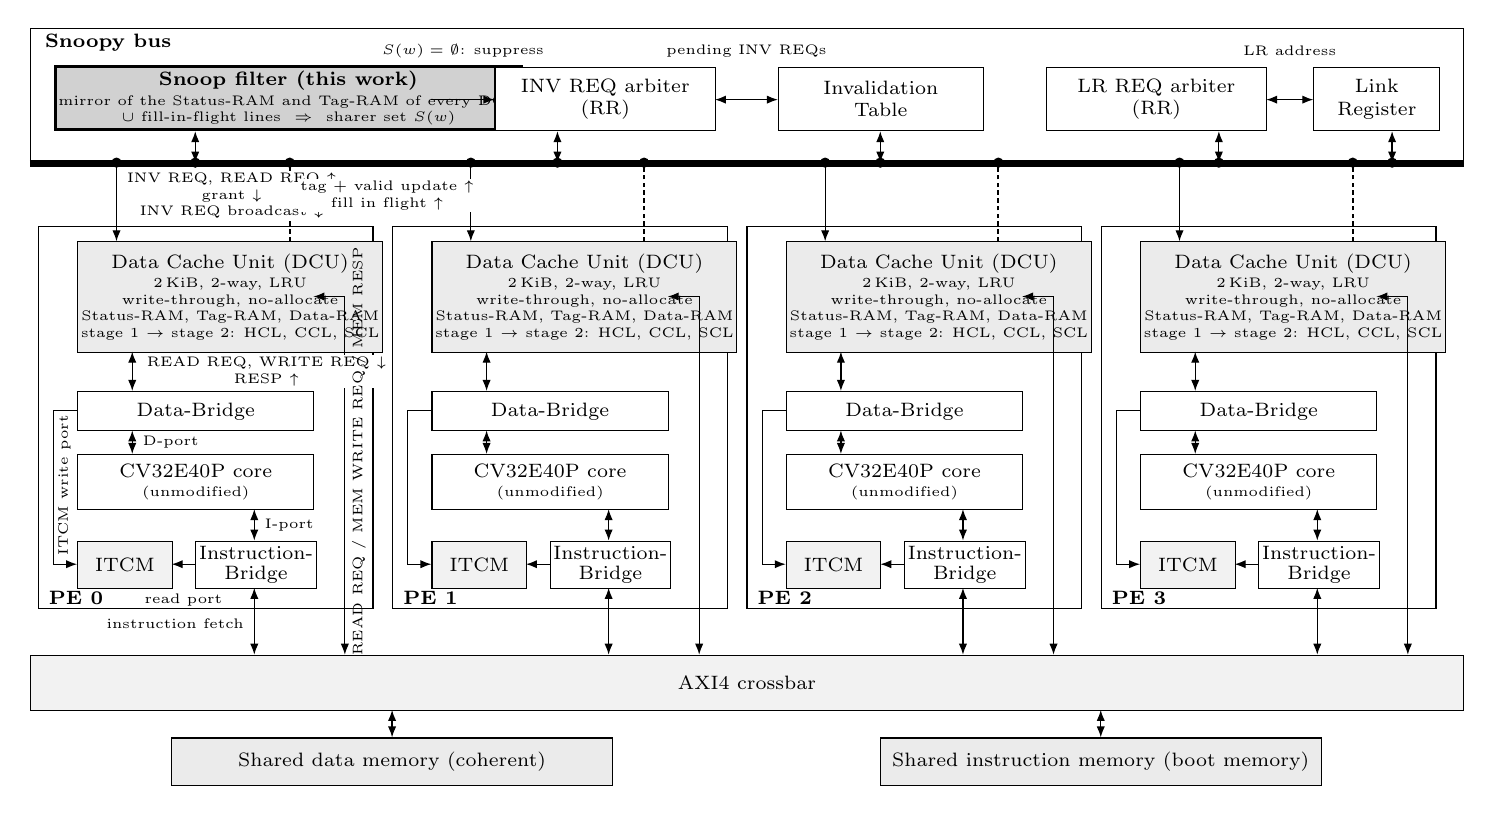
\begin{tikzpicture}[
  x=1mm, y=1mm, font=\scriptsize,
  box/.style  ={draw,rectangle,align=center,inner sep=1.2pt},
  blk/.style  ={box,fill=white,minimum width=30mm},
  sub/.style  ={box,fill=black!5},
  dcu/.style  ={box,fill=black!8,minimum width=30mm,minimum height=14mm},
  pe/.style   ={draw,rectangle,inner sep=0},
  unit/.style ={box,fill=white,minimum height=8mm},
  new/.style  ={box,fill=black!18,line width=1.1pt,minimum height=8mm},
  mem/.style  ={box,fill=black!8,minimum height=6mm,minimum width=56mm},
  bi/.style   ={draw,{Latex[length=1.4mm]}-{Latex[length=1.4mm]},line width=0.45pt},
  ln/.style   ={draw,-{Latex[length=1.4mm]},line width=0.45pt},
  tap/.style  ={draw,{Latex[length=1.4mm]}-,line width=0.45pt},
  mir/.style  ={draw,dashed,dash pattern=on 1.6pt off 1.2pt,line width=0.7pt},
  bus/.style  ={draw,line width=1.6pt},
  dot/.style  ={circle,fill=black,inner sep=0,minimum size=1.3mm},
  lab/.style  ={font=\tiny,inner sep=0.8pt,fill=white,align=center},
  labr/.style ={font=\tiny,inner sep=0.4pt,rotate=90,anchor=center},
]

% ------------------------------------------------------------ processing elements
% x0 = left edge of the PE's components; PE frame runs from x0-2 to x0+39.
\foreach \i/\xo in {0/2, 1/47, 2/92, 3/137} {
  % frame and name
  \node[pe,minimum width=42.5mm,minimum height=48.5mm,anchor=north west]
        (pe\i) at (\xo-2, 2) {};
  \node[font=\scriptsize\bfseries,anchor=west,inner sep=1pt] at (\xo-1, -45.3) {PE \i};

  % blocks, top to bottom
  \node[dcu,anchor=north west] (d\i) at (\xo+3, 0)
    {Data Cache Unit (DCU)\\[-1pt]
     {\tiny 2\,KiB, 2-way, LRU}\\[-2pt]
     {\tiny write-through, no-allocate}\\[-2pt]
     {\tiny Status-RAM, Tag-RAM, Data-RAM}\\[-2pt]
     {\tiny stage 1 $\rightarrow$ stage 2: HCL, CCL, SCL}};
  \node[blk,minimum height=5mm,anchor=north west] (db\i) at (\xo+3, -19) {Data-Bridge};
  \node[blk,minimum height=7mm,anchor=north west] (c\i)  at (\xo+3, -27) {CV32E40P core\\[-1pt]{\tiny (unmodified)}};
  \node[sub,minimum width=12mm,minimum height=6mm,anchor=north west] (it\i) at (\xo+3, -38) {ITCM};
  \node[blk,minimum width=15mm,minimum height=6mm,anchor=north west] (ib\i) at (\xo+18, -38) {Instruction-\\[-1pt]Bridge};

  % core data port: DCU <-> Data-Bridge <-> core  (channel at x0+19)
  \draw[bi] (\xo+10, -14) -- (\xo+10, -19);
  \draw[bi] (\xo+10, -24) -- (\xo+10, -27);
  % core instruction port: core -> Instruction-Bridge -> shared instr. memory
  \draw[bi] (\xo+25.5, -34) -- (\xo+25.5, -38);
  \draw[bi] (\xo+25.5, -44) -- (\xo+25.5, -52.5);
  % Instruction-Bridge -> ITCM read port
  \draw[ln] (\xo+18, -41) -- (\xo+15, -41);
  % Data-Bridge -> ITCM write port, along the left edge of the PE
  \draw[ln] (\xo+3, -21.5) -- (\xo, -21.5) -- (\xo, -41) -- (\xo+3, -41);
  % DCU <-> AXI4 crossbar, along the right edge of the PE
  \draw[bi] (\xo+33, -7) -- (\xo+37, -7) -- (\xo+37, -52.5);
  % taps into the snoopy bus: requests/grants (solid), mirror updates (dashed)
  \draw[tap] (\xo+8, 0) -- (\xo+8, 10);   \node[dot] at (\xo+8, 10) {};
  \draw[mir] (\xo+30, 0) -- (\xo+30, 10); \node[dot] at (\xo+30, 10) {};
}

% labels, written once on PE 0 (every PE is wired identically)
\node[lab,anchor=west] at (13.5, -16.5) {READ REQ, WRITE REQ $\downarrow$\\RESP $\uparrow$};
\node[lab,anchor=west] at (13, -25.5) {D-port};
\node[lab,anchor=west] at (28.5, -36) {I-port};
\node[lab] at (18.5, -45.5) {read port};
\node[labr] at (3.4, -31) {ITCM write port};
\node[labr] at (40.8, -30) {MEM READ REQ / MEM WRITE REQ / MEM RESP};
\node[lab,anchor=east] at (26.5, -48.5) {instruction fetch};
\node[lab,anchor=west] at (11, 5.8)
  {INV REQ, READ REQ $\uparrow$\\grant $\downarrow$\\INV REQ broadcast $\downarrow$};
\node[lab,anchor=west] at (33, 5.8)
  {tag + valid update $\uparrow$\\fill in flight $\uparrow$};

% ------------------------------------------------------------------ snoopy bus
\node[pe,minimum width=182mm,minimum height=17.5mm,anchor=south west] at (-1, 9.5) {};
\node[font=\scriptsize\bfseries,anchor=west,inner sep=1pt] at (0.5, 25.3) {Snoopy bus};
\draw[bus] (-1, 10) -- (181, 10);

\node[new,minimum width=48mm,anchor=south west] (filt) at (2, 14)
  {\textbf{Snoop filter (this work)}\\[-1pt]
   {\tiny mirror of the Status-RAM and Tag-RAM of every DCU}\\[-2pt]
   {\tiny $\cup$ fill-in-flight lines\ \ $\Rightarrow$\ \ sharer set $S(w)$}};
\node[unit,minimum width=28mm,anchor=south west] (arb1) at (58, 14)  {INV REQ arbiter\\(RR)};
\node[unit,minimum width=26mm,anchor=south west] (itab) at (94, 14)  {Invalidation\\Table};
\node[unit,minimum width=28mm,anchor=south west] (arb2) at (128, 14) {LR REQ arbiter\\(RR)};
\node[unit,minimum width=16mm,anchor=south west] (lreg) at (162, 14) {Link\\Register};

% stubs from the bus line to each component
\foreach \x in {20, 66, 107, 150, 172} {
  \draw[bi] (\x, 10) -- (\x, 14); \node[dot] at (\x, 10) {};
}
% only adjacent components are joined, so nothing crosses
\draw[ln] (50, 18) -- (58, 18);
\node[lab] at (54, 24.2) {$S(w)=\emptyset$: suppress};
\draw[bi] (86, 18) -- (94, 18);
\node[lab] at (90, 24.2) {pending INV REQs};
\draw[bi] (156, 18) -- (162, 18);
\node[lab] at (159, 24.2) {LR address};

% ------------------------------------------------------- crossbar and memories
\node[box,fill=black!5,minimum width=182mm,minimum height=7mm,anchor=north west]
  (xbar) at (-1, -52.5) {AXI4 crossbar};
\node[mem,anchor=north] (sdm) at (45, -63)  {Shared data memory (coherent)};
\node[mem,anchor=north] (sim) at (135, -63) {Shared instruction memory (boot memory)};
\draw[bi] (45, -59.5) -- (45, -63);
\draw[bi] (135, -59.5) -- (135, -63);

\end{tikzpicture}
\end{document}
